\section{Funcionalidades}

No \calopsita{}, também por sua arquitetura de \textit{plugins}, as funcionalidades estão separadas em duas grandes partes: o núcleo e os \textit{plugins}. A primeira, contém apenas partes diretamente relacionadas com desenvolvimento ágil, no sentido mais amplo e irrestrito do termo -- sem interferência de metodologias, seus métodos e métricas. Essas partes variáveis de cada projeto ou dependente de metodologia são deixadas para os \textit{plugins}, que dão ao sistema uma melhor adaptabilidade.

\subsection{Calopsita \textit{Core}}

As funcionalidades que fazem parte do núcleo do \calopsita{} consistem da criação e administração de usuários, projetos, cartões e iterações. Parece ser um núcleo minimal e essa é a intenção, contudo a proposta dos cartões é um tanto diferente e precisa ser explicada. Também faz parte do núcleo toda a infraestrutura necessária para a integração de um plugin ao sistema.

\subsubsection*{Cartões}

Diferente de outros sistemas com o mesmo propósito, o \calopsita{} não possui o conceito de histórias, mas apenas de cartões. Isso foi feito pensando em trazer maior grau de customização para os usuários. Cada cartão pode ter subcartões e o que define a funcionalidade desse cartão é o conjunto de \textit{gadgets} que ele possui. 

A vantagem é que pode-se criar uma hierarquia, tão profunda quanto se desejar, para organizar tudo o que há para ser feito em um projeto. Isso também permite que o projeto possa ser visto no nível de detalhe mais apropriado pra cada envolvido no projeto, seja ele gerente, desenvolvedor ou cliente. 

\begin{figure}[H]
  \centering
  \fbox{
    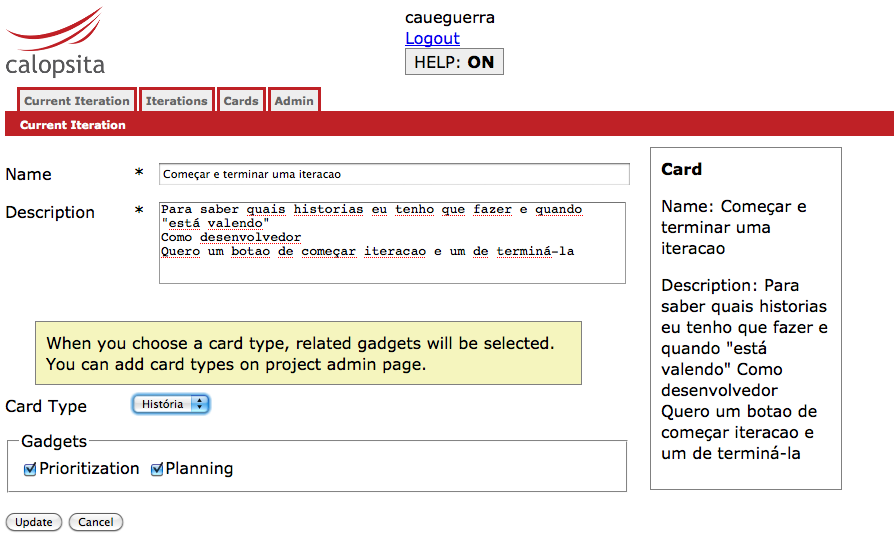
\includegraphics[width=110mm]{images/cartao.png}
  }
  \caption{Cartão}\label{figura:cartao}
\end{figure}

\begin{figure}[H]
  \centering
  \fbox{
    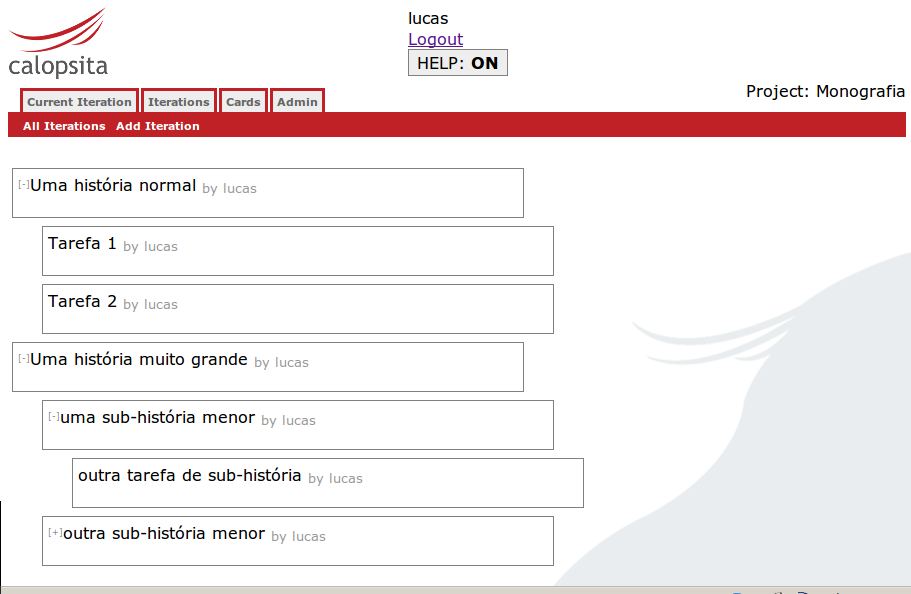
\includegraphics[width=110mm]{images/hierarquia-de-cartoes.png}
  }
  \caption{Cartões mostrados hierarquicamente}\label{figura:hierarquia}
\end{figure}

\subsubsection*{Tipos de Cartões}

Um tipo de cartão é, para o \calopsita{}, um agrupamento de \textit{gadgets} que definem o comportamento de um determinado cartão. Perceba que a noção é puramente semântica, já que os \textit{gadgets} podem ser habilitados e desabilitados individualmente, por cartão.

\begin{figure}[H]
  \centering
  \fbox{
    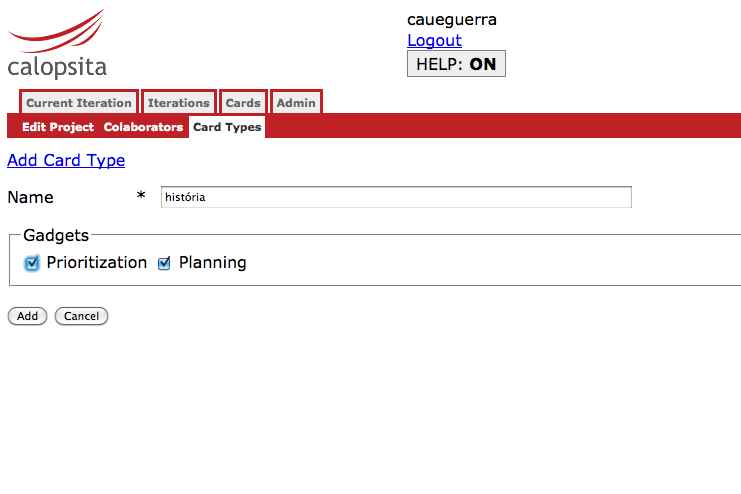
\includegraphics[width=110mm]{images/tipo_cartao.png}
  }
  \caption{Tipos de Cartões}\label{figura:tipo_cartao}
\end{figure}


Está previsto para também fazer parte do núcleo do \calopsita{} uma funcionalidade de histórico de mudanças. Assim, vai ser possível coletar informações para gerar gráficos, e criar um serviço que retorne as últimas modificações feitas, em formato RSS para que os membros do projeto possam utilizar agregadores para acompanhar o andamento da iteração.

\subsection{Calopsita Plugins}

Como explicado anteriormente, o \calopsita{} possuí um núcleo com as funcionalidades essenciais e as demais serão fornecidas através de \textit{plugins}. Temos em nosso \textit{backlog}, diversos plugins para serem implementados e que já viriam na instalação padrão do \calopsita{}. Segue abaixo uma breve descrição de cada um deles:

\begin{itemize}
	\item{Priorização: permite seja atribuída uma prioridade a um determinado cartão através de uma interface baseada em \textit{drag 'n' drop}. Esse plugin já está implementado.
	
	\begin{figure}[H]
	  \centering
	  \fbox{
	    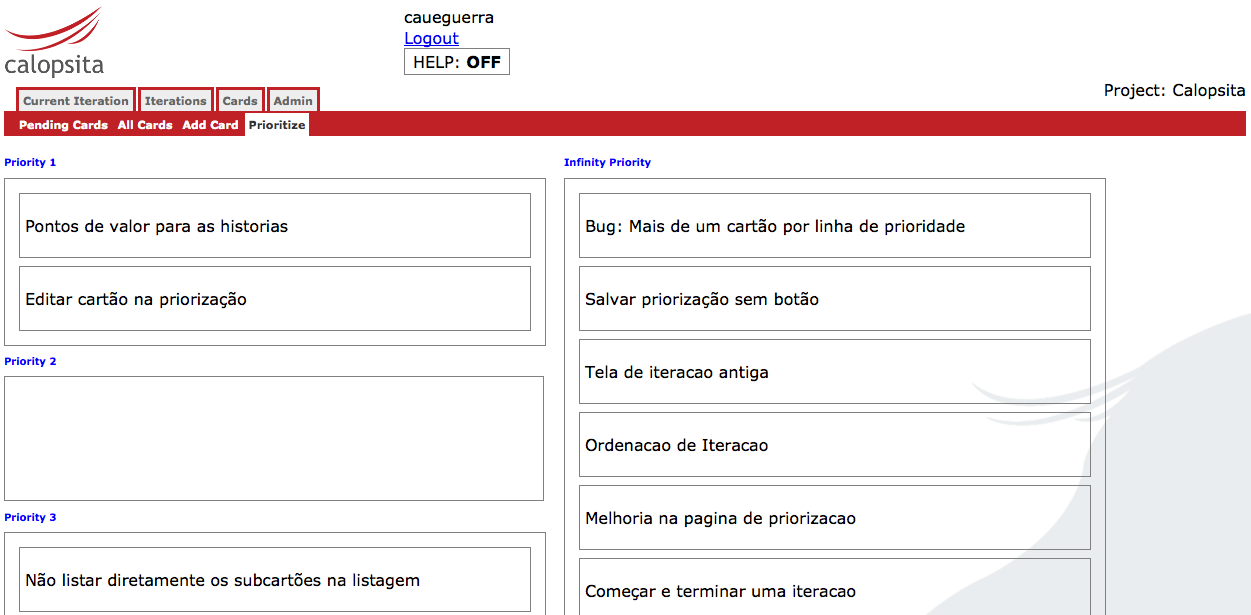
\includegraphics[width=110mm]{images/priorizacao.png}
	  }
	  \caption{Priorizacao}\label{figura:priorizacao}
	\end{figure}
	}
	\item{Planejamento: permite que cartões sejam adicionadas ou removidas de uma determinada iteração. Também baseado em \textit{drag 'n' drop} e já está implementado.
	
	\begin{figure}[H]
	  \centering
	  \fbox{
	    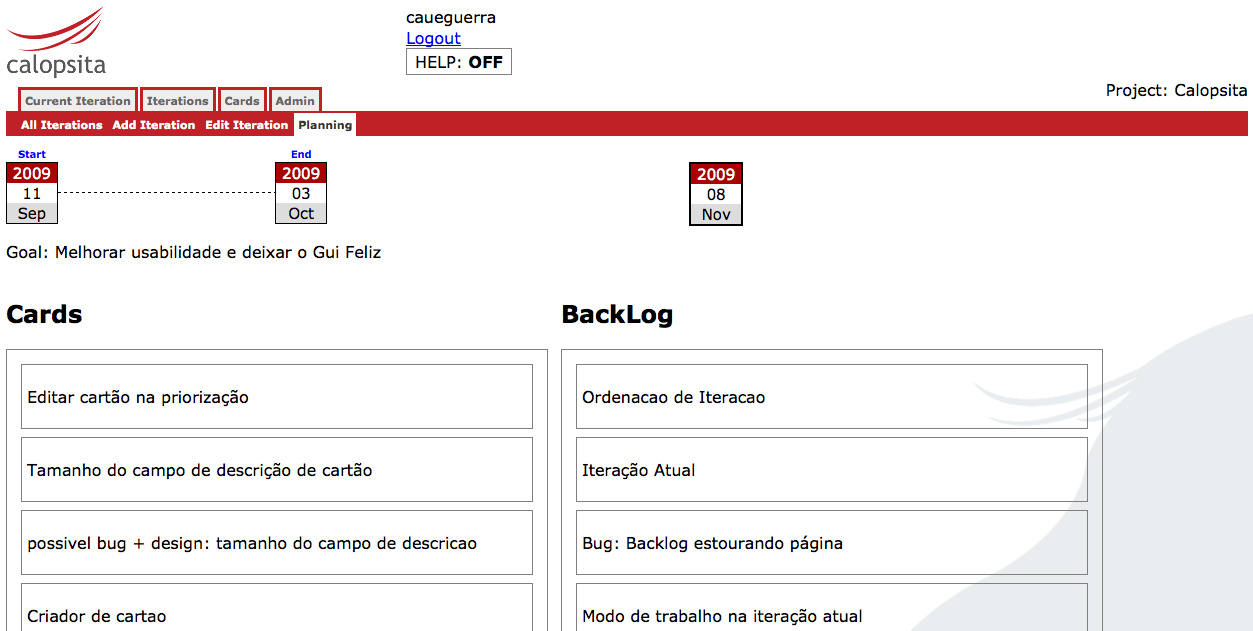
\includegraphics[width=110mm]{images/planejamento.png}
	  }
	  \caption{Planejamento}\label{figura:planejamento}
	\end{figure}
	}
	\item{Gráfico \textit{burn-up}: a idéia desse plugin é que uma nova página contendo o gráfico \textit{burn-up} de uma determinada iteração sejá criada. Este gráfico possui uma linha horizontal, que representa a meta a ser atingida. Essa meta é baseada em alguma métrica da iteração: número de cartões, soma da dificuldade dos cartões, etc. Com o passar dos dias da iteração é marcada a evolução da métrica escolhida, de acordo com o número de cartões prontos.}
	\item{Gráfico \textit{burn-down}: a idéia desse plugin é que uma nova página contendo o gráfico \textit{burn-down} de uma determinada iteração sejá criada. Esse gráfico é parecido com o de \textit{burn-up}, mas a evolução se dá pela quantidade de uma métrica que ainda não está pronta. Geralmente tem uma linha decrescente que representa a velocidade estimada.}
	\item{Marcação de horas: esse plugin permitirá que a pessoa que trabalhou na conclusão de determinado cartão possa marcar o número de horas trabalhadas.}
	\item{Estimativas: possibilitará que um cartão tenha sua dificuldade estimada em pontos.}
	\item{Personas: criará uma área especial para a definição de personas. Essas personas poderão ser utilizadas mais facilmente na criação de novos cartões.}
	\item{Integração com GitHub: permitírá que comentários feitos no \textit{commit} do projeto no GitHub consigam mover cartões dentro de uma determinada iteração e mudar seu status.}
	\item{Modelos de metodologias: ser possível criar modelos com tipos de cartão, nomenclaturas e \textit{gadgets} habilitados que são específicos de uma metodologia. Por exemplo um modelo Scrum teria os tipos de cartão ``História'', ``Épico'' e ``Tarefa'', a iteração se chamaria ``Sprint'' e teria uma ``Meta'', o \textit{Kanban} com as colunas ``Parado'', ``Em Andamento'', ``Em inspeção'' e ``Pronto'', etc.  }
\end{itemize}
